
\section{Fully leptonic results}

\subsection*{Electroweak singlet results}
The final binned fit is performed using the $m_T^I$ histogram for all signals and the number of events for the backgrounds.
For the oppiste-flavour and same-flavour analysis, for every categories and for every mass point from
200\GeV up to 3\TeV the significance  and the 95\% CL
upper exclusion limit are calculated.
The expected final limit from the combination of the opposite and same flavour analysis are shown in Fig.~\ref{fig:lim_OFSF_comb}. 
The SM fraction among gluon gluon fusion and VBF mechanism production is considered.
This limit evaluated represent a considerable improvement respect to the high mass search done with 2015 data 
and the expected and observed limits are compatible with the ATLAS results for a similar analysis, Sec~\ref{NSP} .\\
\begin{figure}[htb]
\centering
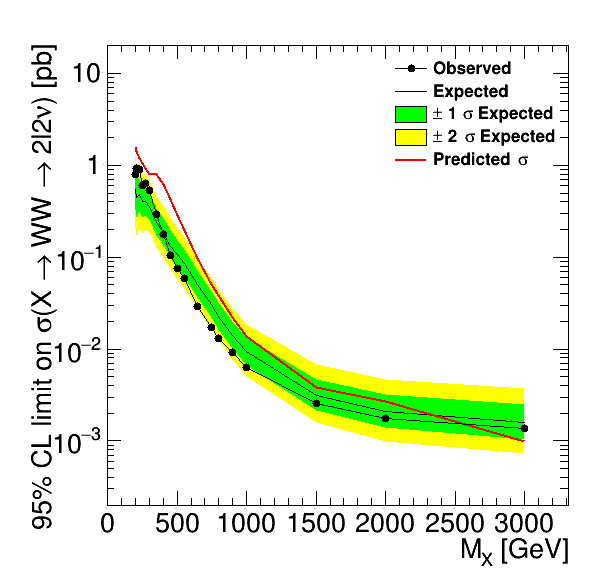
\includegraphics[width=0.65\textwidth]{../AN/Figs/unblinding/Limits/c2_FullComb_unbl.png}
\caption{95$\%$ CL exclusion limits,  on the production gluon gluon fusion and VBF cross section times branching fraction as a function of the mass for the  combination of the two analysis opposite and same flavour, in the full mass range.  The red line represent the predicted cross-section for EW high mass bosons.}
\label{fig:lim_OFSF_comb}
\end{figure}


\subsection*{2HDM results}
In Fig. ~\ref{fig:MSSM} the exclusion limits are shown for the $m_h^{mod+}$ scenario on the left and the hMSSM scenario on the right. The dashed line marks the limit, while the green area shows the side of the limit that is excluded. The bands surrounding the limit indicate the $\pm 1,2\sigma$ contours. For both scenarios the region at low values of $m_{A}$ and $\tan\beta$ is excluded. These results complement well with the exclusion limit given by the MSSM $H\rightarrow\tau\tau$ analysis, where the sensitivity is lower for low $m_{A}$ and $\tan\beta$.

\begin{figure}[htb]
\centering
\subfigure[$m_h^{mod+}$]{
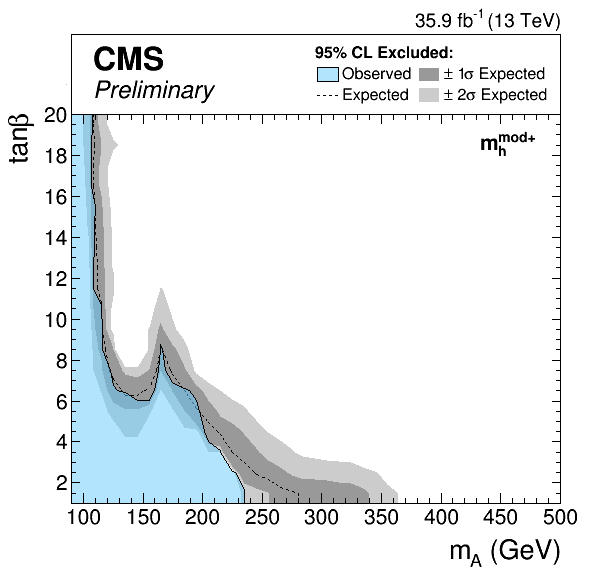
\includegraphics[width=0.45\textwidth]{../AN/Figs/unblinding/2HDM/mhmodp.png}
}
\subfigure[hMSSM]{
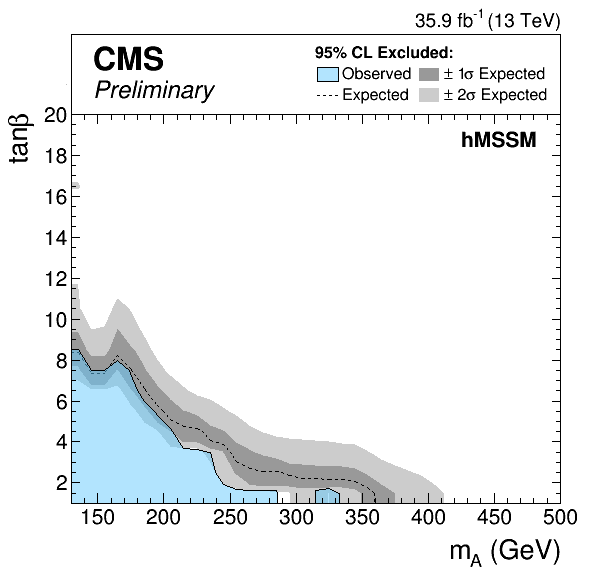
\includegraphics[width=0.45\textwidth]{../AN/Figs/unblinding/2HDM/hmssm.png}
}

\caption{95$\%$ CL exclusion limits on the MSSM $m_h^{mod+}$ scenario (left) and the hMSSM scenario (right).}
    \label{fig:MSSM}
\end{figure}
In Fig. ~\ref{fig:2HDM1} and ~\ref{fig:2HDM2} the exclusion limits are shown for a 2HDM. The limits in ~\ref{fig:2HDM1} for both a type-1 and type-2 2HDM is displayed in a $\cos(\beta-\alpha)$-$\tan\beta$ plane, in which the neutral heavy Higgs boson masses are $m_{H}=m_{A}=200$, $300$, $500\,$GeV and the convention $\sin(\beta-\alpha) > 0$ is used. The plots in Fig. ~\ref{fig:2HDM2} show the limit in the $m_{H}$-$\tan\beta$ plane. Here it is again assumed that $m_{H}=m_{A}$ and $\sin(\beta-\alpha) > 0$, but here the relationship between $\beta$ and $\alpha$ is $\cos(\beta-\alpha)=0.1$. 
%The exclusion limits seen here are larger compared to those produced in the similar analysis by ATLAS. A possible reason may be the choice of the discriminating variable $m_{T}^{I}$ or the different categorization.

\begin{figure}[htb]
\centering
\subfigure[Type-1, $m_{H}=200\,$GeV]{
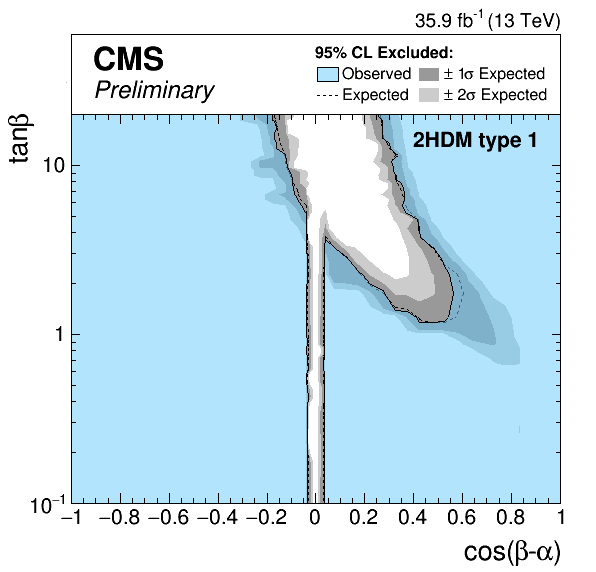
\includegraphics[width=0.45\textwidth]{../AN/Figs/unblinding/2HDM/thdm_cosba_t1_200.png}
}
\subfigure[Type-2, $m_{H}=200\,$GeV]{
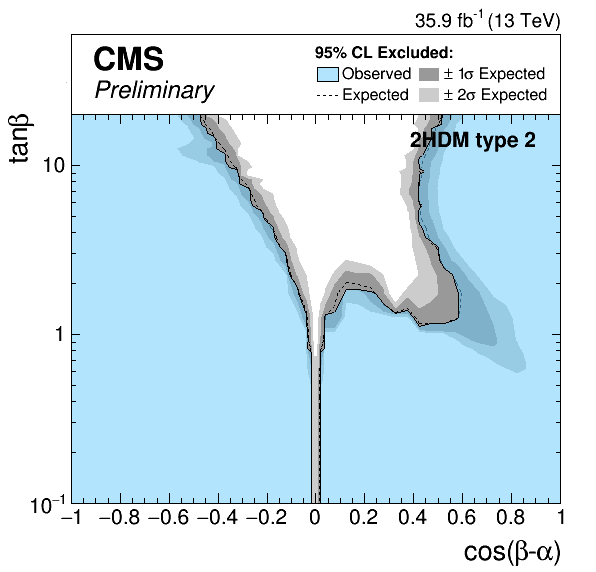
\includegraphics[width=0.45\textwidth]{../AN/Figs/unblinding/2HDM/thdm_cosba_t2_200.png}
}
\\
\subfigure[Type-1, $m_{H}=300\,$GeV]{
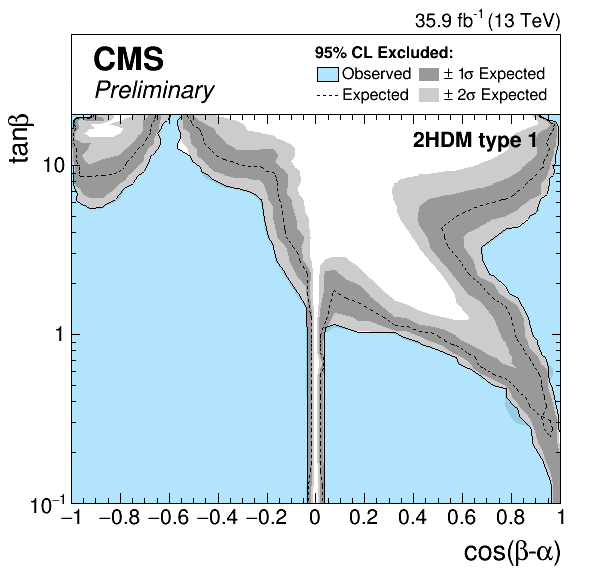
\includegraphics[width=0.45\textwidth]{../AN/Figs/unblinding/2HDM/thdm_cosba_t1_300.png}
}
\subfigure[Type-2, $m_{H}=300\,$GeV]{
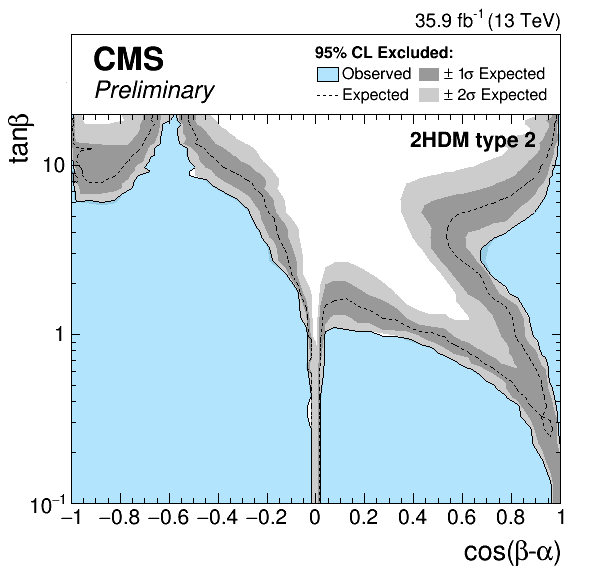
\includegraphics[width=0.45\textwidth]{../AN/Figs/unblinding/2HDM/thdm_cosba_t2_300.png}
}
\\
\subfigure[Type-1, $m_{H}=500\,$GeV]{
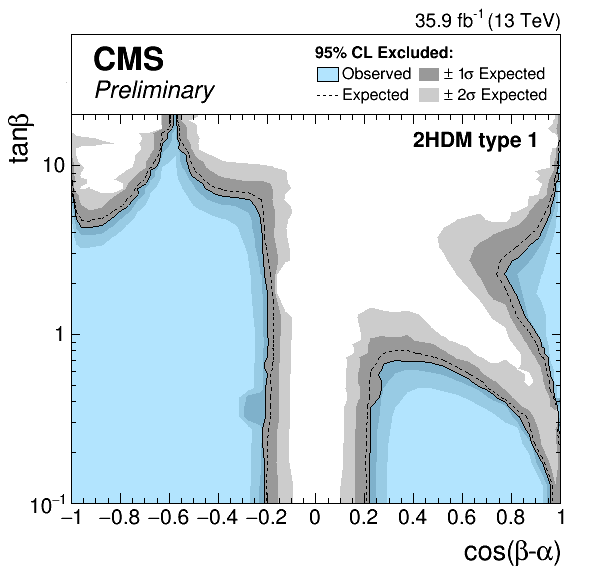
\includegraphics[width=0.45\textwidth]{../AN/Figs/unblinding/2HDM/thdm_cosba_t1_500.png}
}
\subfigure[Type-2, $m_{H}=500\,$GeV]{
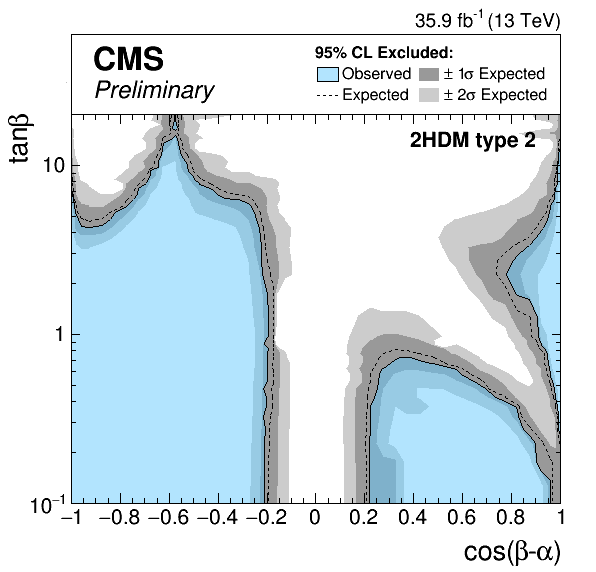
\includegraphics[width=0.45\textwidth]{../AN/Figs/unblinding/2HDM/thdm_cosba_t2_500.png}
}
\caption{95$\%$ CL exclusion limits on a 2HDM with $\cos(\beta-\alpha)$ on the x-axis. Limits are shown for a type-1 and type-2 2HDM for different masses $m_{H}=200$, $300$, $500\,$GeV.}
    \label{fig:2HDM1}
\end{figure}

\begin{figure}[htb]
\centering
\subfigure[Type-1, $\cos(\beta-\alpha)=0.1$]{
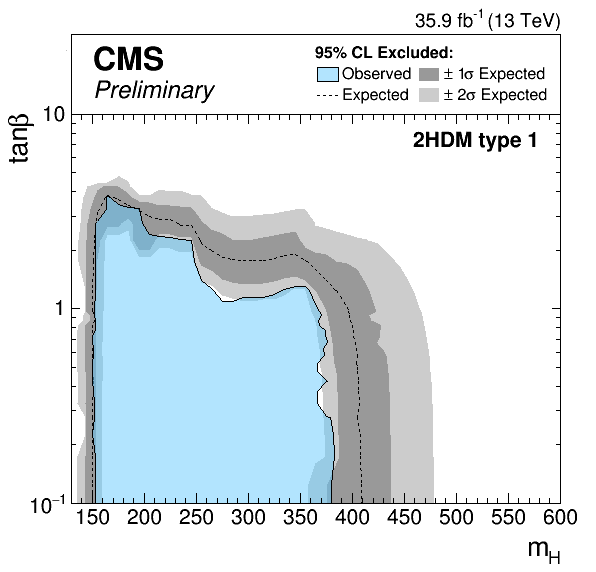
\includegraphics[width=0.45\textwidth]{../AN/Figs/unblinding/2HDM/thdm_mh_t1.png}
}
\subfigure[Type-2, $\cos(\beta-\alpha)=0.1$]{
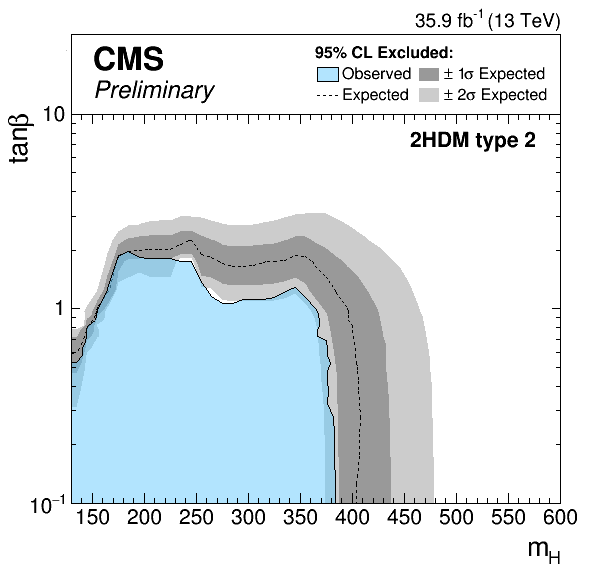
\includegraphics[width=0.45\textwidth]{../AN/Figs/unblinding/2HDM/thdm_mh_t2.png}
}

\caption{95$\%$ CL exclusion limits on a 2HDM with $m_{H}$ on the x-axis. Limits are shown for a type-1 and type-2 2HDM for $\cos(\beta-\alpha)=0.1$.}
    \label{fig:2HDM2}
\end{figure}

\section{Results for the combination of fully- and semi-leptonic analysis}
No evidence for an excess of events with respect to the SM predictions is observed and thus, exclusion
limits in the product of the cross section production of an hypothetical signal times the BR of the decay
to two W bosons is evaluated.
For every mass point from 200 GeV up to 3 TeV the 95\% CL upper exclusion limit are calculated in the
hypothesis that the searched signal has the same width of a SM Higgs boson of corresponding mass.
The expected and observed exclusion limits on the sum of gluon-gluon fusion and VBF cross sections times branching
fraction, assuming that the ratio of cross sections between the two production processes is the same as in
the SM, is shown in Fig.~\ref{lim_superC}, corresponding to the combination of the fully-leptonic and semi-leptonicanalysis.
This result represents a very big improvements in for the high mass searches. 
In addition it enhances the upper limits of a factor of $\sim$10 at low mass and $\sim$100 at high mass the ATLAS limits evaluated at $\sqrt{s}=13$ TeV using partially 2016 data, Fig.~\ref{ATLAS-CONF-2016-074_fig}.
The value of upper limit are comparable with the results obtained in CMS for $X \to ZZ$ with final state ($4\ell$, $2\ell 2\nu$ and $2\ell 2q$) \cite{Sirunyan:2018qlb}.\\
\newline
The production of the $X$ resonance has been considered to be either in gluon gluon fusion and in Vector
Boson Fusion with the assumption of the SM fraction. 
However a scan of the fraction of VBF mechanism
production ( $f_{VBF}$ ) is performed to evaluate the upper limits. 
So that parameter, is the fraction of the EW production cross section with respect to the total cross section and the gluon-gluon fusion cross
section is $\sigma_X \times ( 1-  f_{VBF} )$ . Three different values of  $f_{VBF}$ are studied:   $f_{VBF}$ free to floating, $f_{VBF}=$ 0 and $f_{VBF}=$ 1. 
The upper limits for three cases are shown in Fig.~\ref{wwe}  for the combination of the two different analysis.
\begin{figure}[htb]
\centering
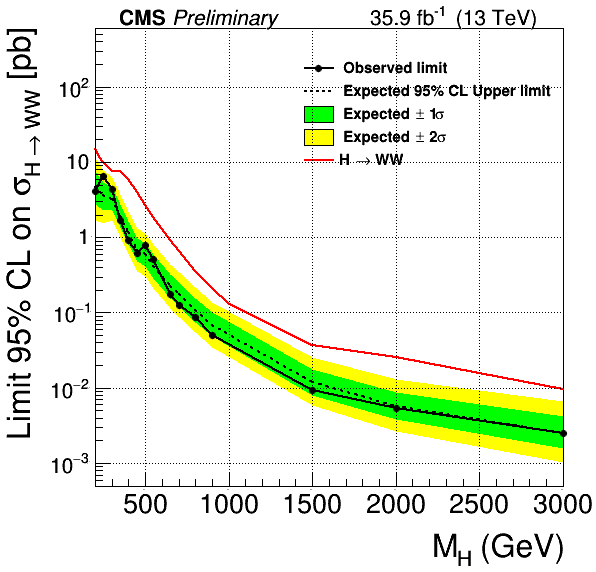
\includegraphics[width=0.65\textwidth]{../Cap6/all}
\caption{Expected and observed exclusion limits at 95\% CL on the sum of ggH and VBF cross
sections times branching fraction for the combination of all the analysis categories as a function
of the resonance mass. The black dotted line corresponds to the central expected value while
the yellow and green bands represent the $\pm 1 \sigma$ and $\pm 2 \sigma$ uncertainties respectively.}
\label{lim_superC}
\end{figure}
\begin{figure}[htb]
\centering
\subfigure[ $f_{VBF}=$ free to float ]{
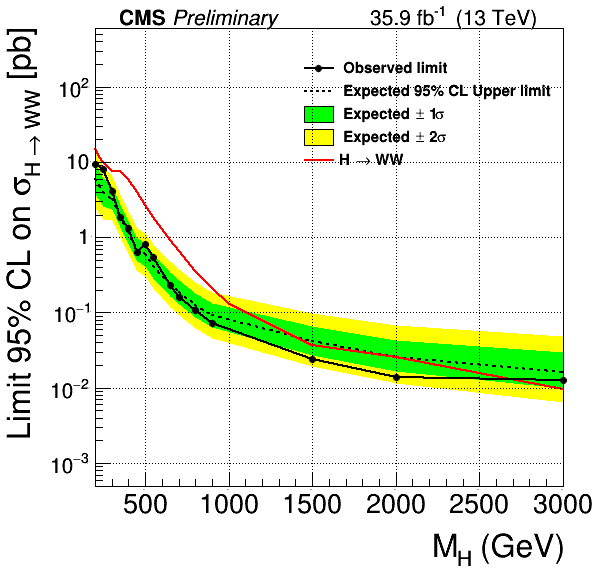
\includegraphics[width=0.45\textwidth]{../Cap6/vbfX}
}
\subfigure[ $f_{VBF}=$0 ]{
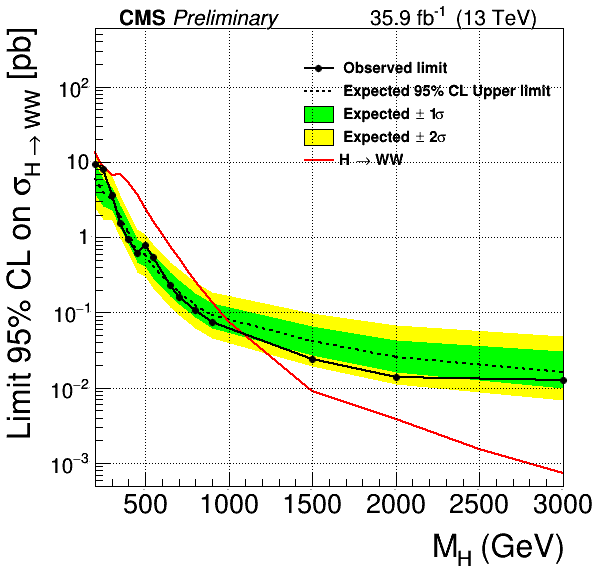
\includegraphics[width=0.45\textwidth]{../Cap6/vbf0}
}
\subfigure[ $f_{VBF}=$ 1]{
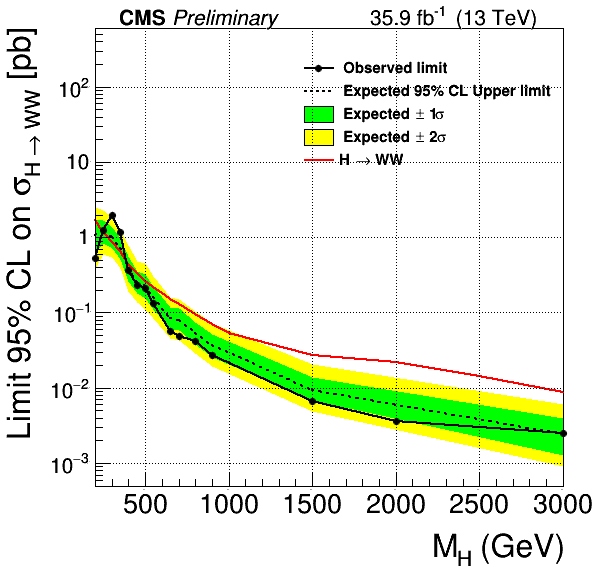
\includegraphics[width=0.45\textwidth]{../Cap6/vbf1}
}
\caption{95\ CL exclusion limits, on the production gluon-gluon fusion and VBF cross section times branching 
for differents $f_{VBF}$ fraction. The red line represent the predicted cross-section for EW high
mass bosons in the free floating case (a), only the predicted vector boson cross-section in
 $f_{VBF}$ case (b) and only the predicted gluon-gluon fusion cross-section in $f_{VBF}$ case (c).}
    \label{wwe}
\end{figure}
